\documentclass[a4paper]{article}

\usepackage{fullpage}
\usepackage[utf8]{inputenc}
\usepackage[T1]{fontenc}
\usepackage[francais]{babel}
\usepackage{listings}
\usepackage{graphicx}
\usepackage{hyperref}

\lstset{
	language=C++,
	basicstyle=\ttfamily,
	showstringspaces=false
}

\author{Titou}
\date{\today}
\title{Compiler du C++}

\begin{document}
\maketitle

\section{Distinction entre les fichiers}
Les fichiers .hpp sont appelés \textbf{fichiers headers}, les fichier .cpp les \textbf{fichiers d'implémentation}. 

\paragraph{Le rôle des headers} est de déclarer l'interface, c'est à dire présenter les types de données et les signatures de variables/fonctions\footnote{La distinction importe peu: en C/C++, un nom de fonction est en fait une variable de type \texttt{pointeur sur fonction} qui pointe sur la première instruction de la fonction.} à l'utilisateur \textit{(ie c'est d'habitude là qu'on met la documentation)}, mais surtout au compilateur, qui pourra savoir si un type de donnée/variable/fonction existe ou non.

\paragraph{Les fichiers d'implémentation} contiennent quant à eux le code des fonctions. Pour utiliser des variables/fonctions définies ailleurs (librairie standard, autre fichier, ...), ils ont besoin de connaître la signature de cette variable. Ils pourront la connaître en incluant le fichier header la contenant. Exemple:
\begin{lstlisting}
#include <cstring>

int main(int argc, const char **argv){
  const char *origine = "Hello world";
  char copie[12];
  
  /* La fonction strcpy, qui copie une chaine dans une autre
     est declaree dans cstring. Le code qui la fait tourner se
     trouve lui dans la librairie standard. */
  strcpy(copie, origine);
  
  return 0;
}
\end{lstlisting}

\section{Etapes de compilation}
Quand on compile, on peut distinguer 3 grandes étapes (il y en a plus):

\begin{figure}[h]
	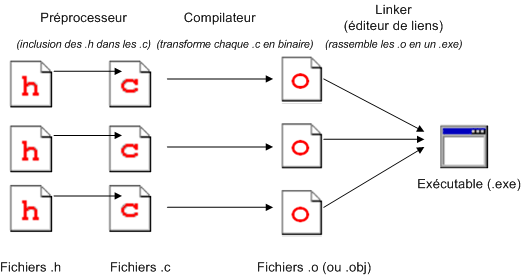
\includegraphics[width=0.75\textwidth]{compilateur.png}
	\caption{Source: Tutoriel C du Site du Zéro}
\end{figure}

\subsection{Préprocesseur} 
Toutes les directives de prérocesseur sont executées: les \lstinline{#include} sont remplacés par le contenu du fichier qu'ils incluent, les valeurs définie par \lstinline{#define} sont remplacées, ...
\paragraph{Types d'erreurs rencontrées à cette étape} 
\begin{itemize}
	\item \texttt{file XXX.hpp not found}
	\item \texttt{Error in macro}
\end{itemize}
\paragraph{Exécuter juste cette étape:} 
\lstinline{$ g++ -E fichierEntree.cpp -o fichierSortie.ii}

\subsection{Compilation et assemblage}
Un fichier d'implémentation est ensuite transformé: les instructions C sont transformées en instructions machine. Le fichier résultant n'est pas encore tout à fait exécutable, on l'appelle \textbf{fichier objet}, et il porte généralement l'extension \textbf{.o}
\paragraph{Types d'erreurs rencontrées à cette étape}
\begin{itemize}
	\item \texttt{syntax error}
	\item \texttt{... was not declared in this scope}
	\item \texttt{expected ... }
	\item \texttt{unknow type or identifier}
\end{itemize}
\paragraph{Exécuter juste cette étape:} 
\lstinline{$ g++ -c fichierEntree.cpp -o fichierSortie.o}

\subsection {Edition des liens}
Enfin, différents fichiers objet sont rassemblés ensemble en un seul \textbf{fichier exécutable}, le programme final. Pour ce faire, toutes les variables/fonctions dont les signatures ont été incluses grâce aux fichiers headers sont remplacées par leur adresse dans le programme.
\paragraph{Types d'erreurs rencontrées à cette étape}
\begin{itemize}
	\item \texttt{Undefined reference to ...}
\end{itemize}
\paragraph{Exécuter juste cette étape:} 
\lstinline{$ g++ fichiersObjets -o fichierExecutable}

\subsection{Raccourcis}
\lstinline{g++} permet d'exécuter les 3 étapes en une seule, ainsi on peut très bien écrire, par exemple: \\
\lstinline{$ g++ -o mainProjLang mainProjLang.cpp Tree.cpp SplitGame.cpp}

\section{Automatisation avec make}
La commande \lstinline{make} sur Linux ou Mac OS X permet d'automatiser le processus de compilation, tout en gardant les fichiers intermédiaire pour ne produire que ceux qui doivent être mis à jour \textit{(si l'heure du fichier de sortie est inférieure à l'heure du fichier d'entrée)}.

Les instructions pour la \textit{recette} finale sont données dans un fichier nommé \textbf{Makefile}. Toutes les étapes ne doivent pas être décrites explicitement, puisque \lstinline{make} \textit{connaît} des règles de base (comme .cpp => .o).

\subsection{Exemple} 
Le fichier Makefile suivant permet, en tapant simplement la commande \lstinline{make} de compiler l'exécutable final mainProjLang. En tapant \lstinline{make test}, et à condition que le fichier test.cpp existe, on construit un executable avec les memes fichiers objets, mais où la fonction \lstinline{main()} vient du fichier test.cpp. Note: les lignes indentées commencent par des tabulations.

\lstinputlisting{Makefile}

\section{Références}
\begin{itemize}
	\item \url{http://www.siteduzero.com/informatique/tutoriels/compilez-sous-gnu-linux}
	\item \url{http://www.gnu.org/software/make/manual/make.html}
	\item A. \bsc{Tannebaum}, Structured Computer Organization, 5\textsuperscript{ème} édition, \textit{Section 7.3: The assembly process}
	\item \url{http://www.siteduzero.com/informatique/tutoriels/apprenez-a-programmer-en-c/la-compilation-separee}
\end{itemize}

\end{document}

